% !TEX root = ../main.tex
%

\chapter{勾配を用いた制約なし最適化}

ここでは,勾配を用いた最適化アルゴリズムをまとめる.

\begin{algorithm}[tp]
    \caption{勾配による最適化}
    \label{alg:optimization_unconstrained_descent-methods_general-descent-method}
    \begin{algorithmic}
        \Procedure{DescentMethod}{$f, \bm{x}_0$}
            \For{$i = 1,2,\ldots$}
                \State 更新方向 $\bm{d}_i \in \setR^n$ を算出する
                \State 直線探索により更新方向に掛ける係数 $t_i$ を決定する
                \Comment{通常 $f(\bm{x}_{i-1} + t_i \bm{d}_i) < f(\bm{x}_{i-1})$ とする}
                \State $\bm{x}_i \gets \bm{x}_{i-1} + t_i \bm{d}_i$
                \If{終了条件を満たしている}
                    \State \Return $\bm{x}_i$
                \EndIf
            \EndFor
        \EndProcedure
    \end{algorithmic}
\end{algorithm}

勾配を用いた最適化アルゴリズムでは,
一般に
Algorithm \ref{alg:optimization_unconstrained_descent-methods_general-descent-method}
のような手順で反復的に最適化を進めていく.
更新方向の算出方法により,
最急降下法,Newton 法,共役勾配法のような様々なアルゴリズムが存在する.

\section{直線探索}

まずは,直線探索の方法をまとめる.
直線探索では
$\nabla f(\bm{x}_{i-1})^\top \bm{d}_i < 0$ となっている
(つまり,$\bm{d}_i$ は目的関数が減少する方向になっている)
ことを前提とする.

直線探索の方法として,以下のような方法が挙げられる.

\begin{itemize}
    \item 厳密直線探索
    \item Backtracking line search
\end{itemize}

厳密直線探索は,更新後の目的関数の値
$f(\bm{x}_{i-1} + t_i \bm{d}_i)$
が最小となる $t_i$ を探索する.

\begin{algorithm}[tp]
    \caption{Backtracking Line Search \cite[Section 9.2]{Boyd2004}}
    \label{alg:optimization_unconstrained_descent-methods_BacktrackingLineSearch}
    \begin{algorithmic}
        \Procedure{BacktrackingLineSearch}{$f, \bm{x}_{i-1}, \bm{d}_i$}
            \State $t_i \gets 1$
            \While{$f(\bm{x}_{i-1} + t_i \bm{d}_i) > f(\bm{x}_{i-1}) + \alpha t_i \nabla f(\bm{x}_{i-1})^\top \bm{d}_i$}
                \State $t_i \gets \beta t_i$
            \EndWhile
        \EndProcedure
    \end{algorithmic}
\end{algorithm}

\begin{figure}[tp]
    \centering
    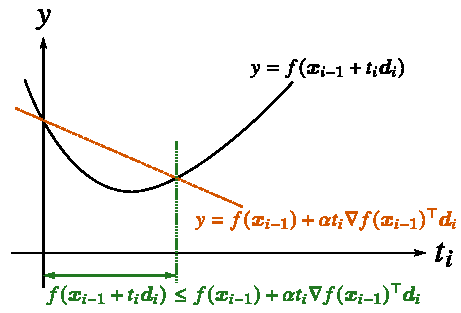
\includegraphics[width=0.7\linewidth]{optimization/Armijo-rule-image.pdf}
    \caption{Armijo の条件(式\eqref{eq:optimization_unconstrained_descent-methods_Armijo-rule})のイメージ}
    \label{fig:optimization_unconstrained_descent-methods_Armijo-rule-image}
\end{figure}

Backtracking Line Search \cite[Section 9.2]{Boyd2004} は
Armijo の条件 \cite[Section 7.5]{Luenberger2003}
\begin{equation}
    f(\bm{x}_{i-1} + t_i \bm{d}_i) \le f(\bm{x}_{i-1}) + \alpha t_i \nabla f(\bm{x}_{i-1})^\top \bm{d}_i
    \label{eq:optimization_unconstrained_descent-methods_Armijo-rule}
\end{equation}
を利用する.
ここで,$\alpha$ は $\alpha \in (0,1)$ を満たす定数であり,
Armijo の条件は,
図\ref{fig:optimization_unconstrained_descent-methods_Armijo-rule-image}のように
十分小さい $t_i$ を選択するための条件となっている.
Backtracking Line Search では,
$\alpha \in (0, 1/2)$ とし,
Algorithm \ref{alg:optimization_unconstrained_descent-methods_BacktrackingLineSearch}
のように
$t_i$ を初期値 1 から $\beta \in (0, 1)$ 倍していき,
式 \eqref{eq:optimization_unconstrained_descent-methods_Armijo-rule} を満たすものを探索する.
一般に,パラメータ $\alpha$, $\beta$ は
$\alpha \in [0.01, 0.3]$, $\beta \in [0.1, 0.8]$ の範囲で設定される
\cite[Section 9.2]{Boyd2004}.

\section{最急降下法}

最急降下法では,更新方向を $\bm{d}_i = -\nabla f(\bm{x}_{i-1})$ とする.
確実に目的関数の減少する方向を示しており,
ここで示す他のアルゴリズムよりも更新方向の算出が簡単である.
目的関数が強凸関数である場合において,
最適解への収束が証明されている
\cite[Section 9.3.1]{Boyd2004}.

\section{Newton 法}

Newton 法では,
目的関数が狭義凸関数である(つまり,Hessian $\nabla^2 f(\bm{x}_{i-1})$ が正定値である)場合を対象とし,
更新方向を
$\bm{d}_i = -\nabla^2 f(\bm{x}_{i-1})^{-1} \nabla f(\bm{x}_{i-1})$
とする.
$\nabla^2 f(\bm{x}_{i-1})$ が正定値である場合,
$\nabla^2 f(\bm{x}_{i-1})^{-1}$ も正定値になる
\footnote{%
対称行列 $A$ が正定値である場合,$A$ の固有値は正の実数である.%
$A$ は固有値分解により $A=VDV^\top$ ($D$ は固有値による対角行列,$V$ は直交行列)と書くことができるため,%
$A^{-1} = VD^{-1}V^\top$ となる.%
よって,$A^{-1}$ の固有値も全て正の実数であり,%
$A^{-1}$ は正定値である.%
}
ため,
最適解でない $\bm{x}_{i-1}$ においては
$\nabla f(\bm{x}_{i-1})^\top \bm{d}_i = -\nabla f(\bm{x}_{i-1})^\top \nabla^2 f(\bm{x}_{i-1})^{-1} \nabla f(\bm{x}_{i-1}) < 0$
となり,目的関数が減少する方向になっていることを確認できる.
Newton 法の収束性については \cite[Section 9.5.3, 9.6.4]{Boyd2004} にて議論されている.

\section{準 Newton 法}

Newton 法では,
Hessian $\nabla^2 f(\bm{x}_{i-1})$ の逆行列が必要になるが,
$x^4$ のように 2 階微分が 0 になる点があったり,
Hessian の逆行列を安定的に計算できない点があったりする場合には使用できない.
そこで,Newton 法の更新方向
$\bm{d}_i = -\nabla^2 f(\bm{x}_{i-1})^{-1} \nabla f(\bm{x}_{i-1})$
における Hessian を
$\bm{d}_i = -H_{i-1} \nabla f(\bm{x}_{i-1})$
のように Hessian の代わりの行列で置き換える準 Newton 法と呼ばれるアルゴリズムがある.

準 Newton 法のうち,
Davidon-Fletcher-Powell (DFP) 公式では次のように $H_i$ を算出する
\cite[Section 9.3]{Luenberger2003}, \cite[Section 10.9]{Press2007}.
\begin{align}
    H_{i+1} &= H_i + \frac{\bm{p}_i \bm{p}_i^\top}{\bm{p}_i^\top \bm{q}_i}
        - \frac{H_i \bm{q}_i \bm{q}_i^\top H_i}{\bm{q}_i^\top H_i \bm{q}_i} \\
    \bm{p}_i &= \bm{x}_{i+1} - \bm{x}_i \\
    \bm{q}_i &= \nabla f(\bm{x}_{i+1}) - \nabla f(\bm{x}_i)
\end{align}
初期値 $H_0$ を対称な正定値の行列にしておけば,
全ての $H_i$ が帰納的に正定値になる
\cite[Section 9.3]{Luenberger2003}.
$H_i$ が正定値であれば,更新方向 $\bm{d}_i$ は目的関数の減少する方向になる.

また,同様の性質を持つ公式の 1 つとして,
Broyden-Fletcher-Goldfarb-Shanno (BFGS) 公式が存在する
\cite[Section 9.4]{Luenberger2003}.
\begin{align}
    H_i &= B_i^{-1} \\
    B_{i+1} &= B_i + \frac{\bm{q}_i \bm{q}_i^\top}{\bm{q}_i^\top \bm{p}_i}
        - \frac{B_i \bm{p}_i \bm{p}_i^\top B_i}{\bm{p}_i^\top B_i \bm{p}_i}
\end{align}
逆行列を計算することで次のようにも書くことができる
\cite[Section 10.9]{Press2007}.
\begin{align}
    H_{i+1} &= H_i + \frac{\bm{p}_i \bm{p}_i^\top}{\bm{p}_i^\top \bm{q}_i}
        - \frac{H_i \bm{q}_i \bm{q}_i^\top H_i}{\bm{q}_i^\top H_i \bm{q}_i}
        + \bm{q}_i^\top H_i \bm{q}_i \bm{v}_i \bm{v}_i^\top \\
    \bm{v}_i &= \frac{\bm{p}_i}{\bm{p}_i^\top \bm{q}_i}
        - \frac{H_i \bm{q}_i}{\bm{q}_i^\top H_i \bm{q}_i}
\end{align}

\section{共役勾配法}

共役勾配法では,
\begin{align}
    \bm{d}_1 &= -\nabla f(\bm{x}_{i-1}) \\
    \bm{d}_i &= -\nabla f(\bm{x}_{i-1}) + \gamma_i \bm{d}_{i-1} \\
    \gamma_i &= 
        \frac{(\nabla f(\bm{x}_{i-1}) - \nabla f(\bm{x}_{i-2}))^\top \nabla f(\bm{x}_{i-1})}
        {\|\nabla f(\bm{x}_{i-2})\|_2^2}
\end{align}
のように更新方向を算出する
\cite[Section 8.6]{Luenberger2003}.
$\gamma_i$ については複数の形式があるが,
ここで示している Polak-Ribiere 法は一般により良い結果が得られるという
\cite[Section 8.6]{Luenberger2003}, \cite[Section 10.8]{Press2007}.
Newton 法では計算量の多い逆行列の計算が必要だが,
共役勾配法では計算量が変数の次元のオーダーに収まるため,
各反復の計算時間を抑えられる.
